\documentclass[../../main.tex]{subfiles}

\begin{document}
\section{Moto Parabolico dei corpi}

\begin{minipage}{0.6\textwidth}
    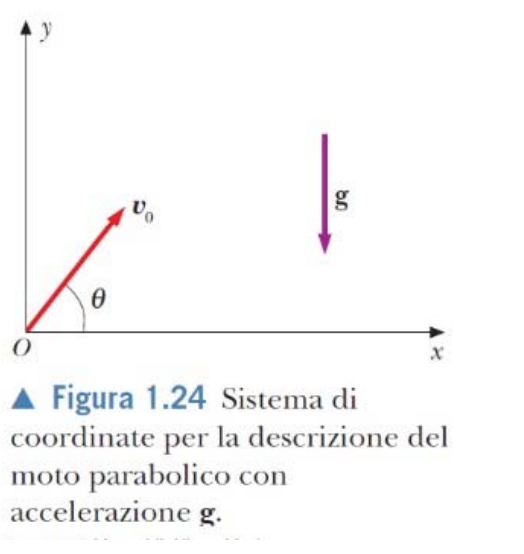
\includegraphics[width=0.5\textwidth]{proiettile1.png}
\end{minipage}
\begin{minipage}{0.4\textwidth}
    \begin{math}
        \bar{a} = -g\bar{u}_z \\
        \bar{v}(t) = \bar v_0 + \int_{0}^{t} \bar{g}dt = \bar{v}_0 - g\bar{u}_z t \\
        \bar v (t) = v_0\cos\theta \cdot \bar u_x + (v_0\sin\theta - gt)\bar u_z \\
        \bar x(t) = \bar x_0 + (v_0\cos\theta)t\bar u_x + (v_0\sin\theta - \dfrac{1}{2}gt^2)\bar u_z
    \end{math}
\end{minipage}

\[
    \textit{Scrittura parametrica: }
    \begin{cases}
        x(t) = (v_0\cos\theta)t \\
        y(t) = v_0\sin\theta t - \dfrac{1}{2}gt^2
    \end{cases}
\]
\[
    t = \dfrac{x}{v_0\cos\theta}
\]
\[
    y(x) = x\tan\theta - \dfrac{gx^2}{2v_0^2\cos^2\theta} \ \ \ \textit{Equazione della traiettoria}
\]
\begin{figure}[h!]
    \centering
    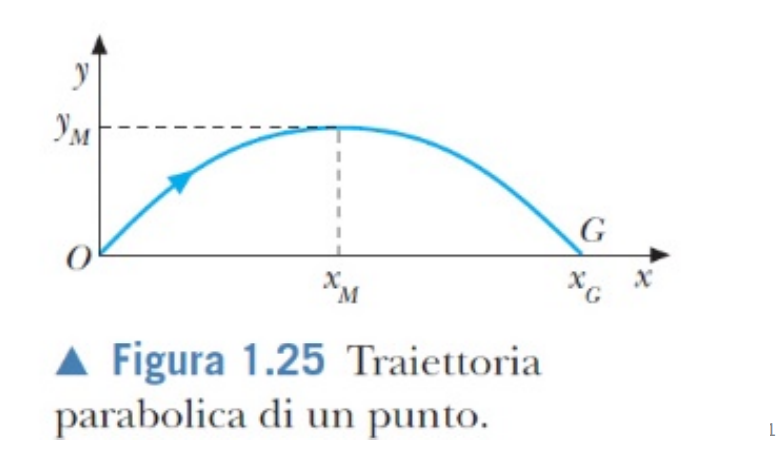
\includegraphics[width=0.5\textwidth]{traiettoriaparabola.png}
    \caption{Traiettoria del moto parabolico}
\end{figure}
\[
    y = 0 \implies x\tan\theta - \dfrac{gx^2}{2v_0^2\cos^2\theta} = 0
\]
RECUPERA 1:27 - 1:35

\subsection{Angoli e gittata}
\begin{figure}[h!]
    \centering
    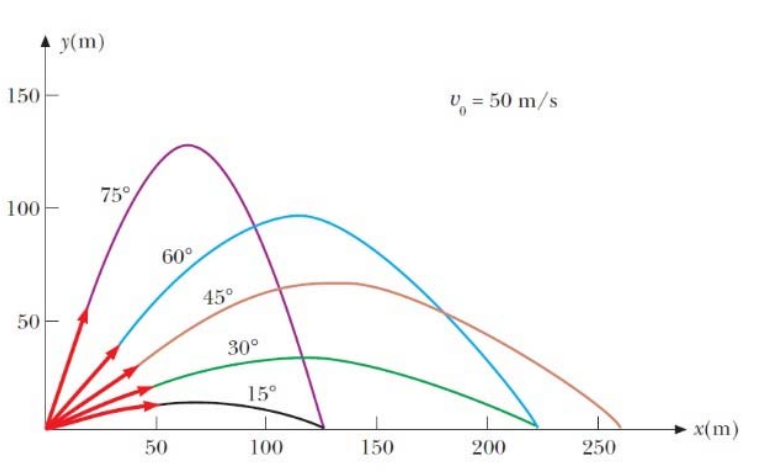
\includegraphics[width=0.5\textwidth]{angoloegittata.png}
\end{figure}
\[
    x_g = \dfrac{2v_0^2\cos\theta\sin\theta}{g} = \dfrac{v_0^2\sin 2\theta}{g} \ \ \ \textit{Gittata}
\]
\[
    \dfrac{dx_g}{d\theta} = \dfrac{2v_0^2(-\sin\theta)\sin\theta}{g} + \dfrac{2v_0^2\cos^2\theta}{g} = \dfrac{2v_0^2}{g}(cos^2\theta - \sin^2\theta) \iff \cos^2\theta = \sin^2\theta \iff \theta = \frac{\pi}{4}
\]
\end{document}